\documentclass[10pt]{beamer}

\usetheme{default} % theme général du diaporama

% paquets pour le français
\usepackage[T1]{fontenc}
\usepackage[utf8]{inputenc}

\title{Présentation - Modèles de distribution d'espèces}
\author{Gabriel Dansereau}

\begin{document}

\begin{frame}
  \titlepage
\end{frame}

\begin{frame}
  \frametitle{Introduction}
  \begin{itemize}
    \item But : ...
    \item Données
    \begin{itemize}
      \item GBIF
      \item eBird
    \end{itemize}
    \item Méthodes
    \begin{itemize}
      \item BIOCLIM
      \item Random Forests
    \end{itemize}
  \end{itemize}
\end{frame}

\begin{frame}
  \frametitle{Données brutes - 1 espèce, beaucoup d'observations}
  \begin{figure}
    \centering
    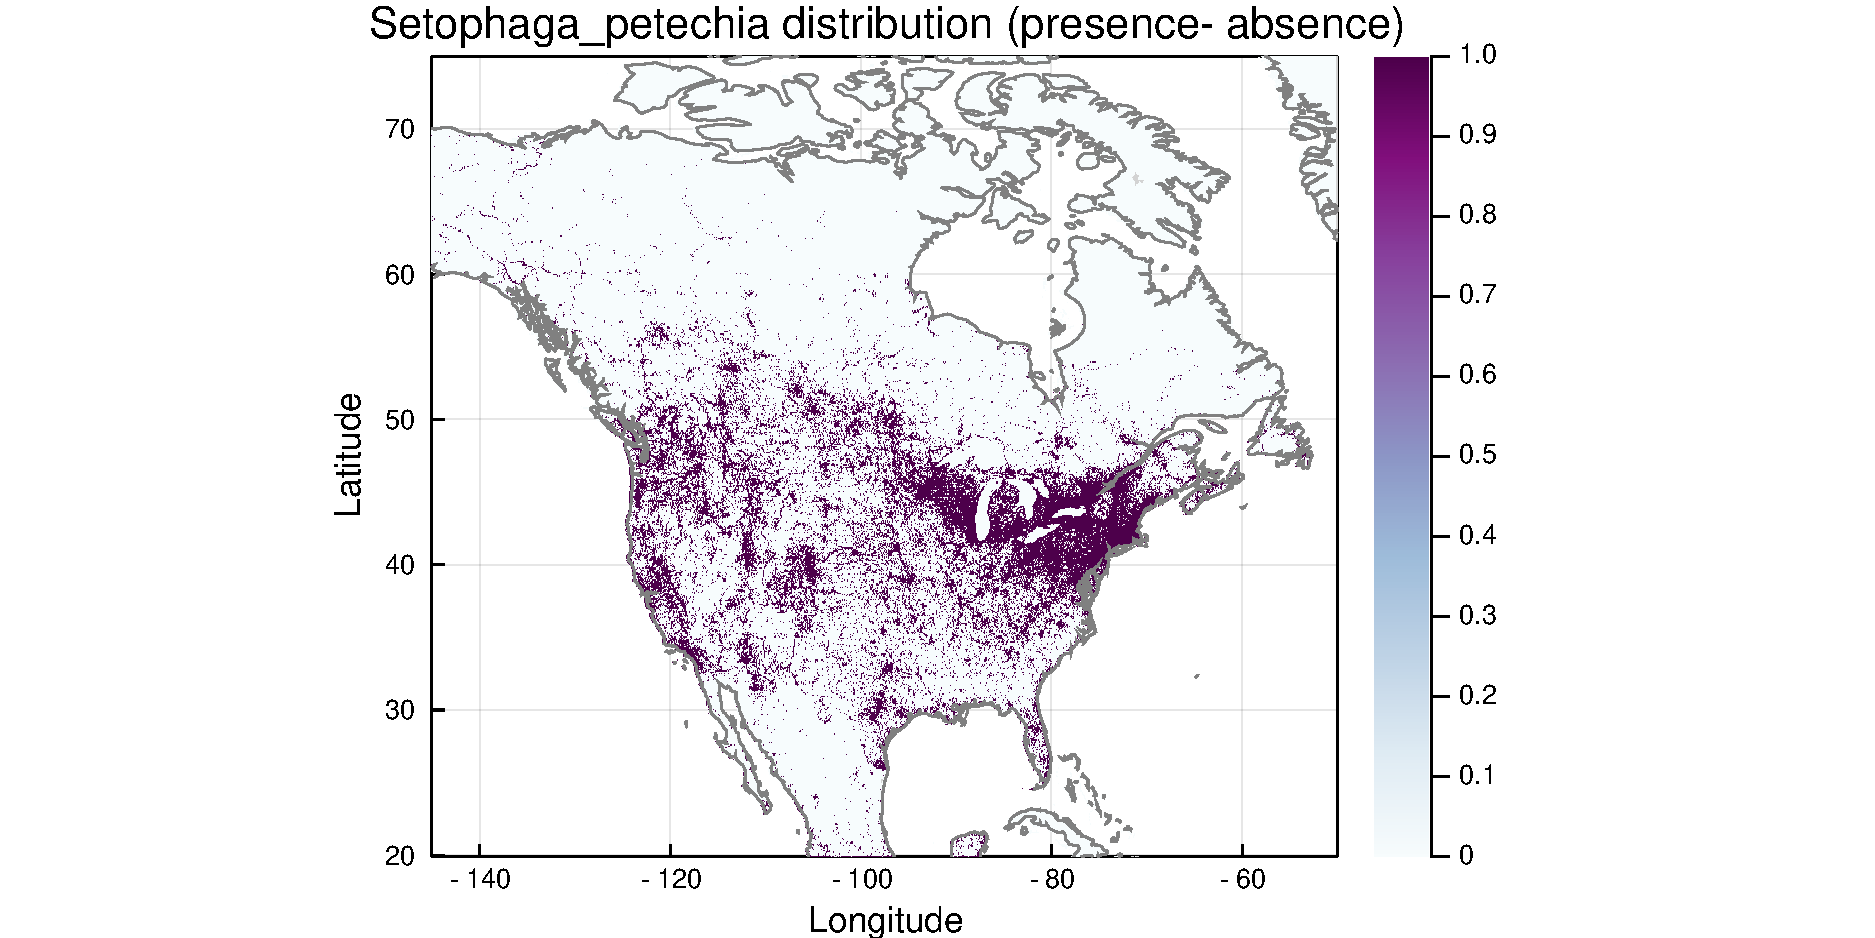
\includegraphics[scale=0.4]{fig/raw-sp-Setophaga_petechia.pdf}
    \caption{Distribution des observations de la Paruline jaune (présence-absence)}
  \end{figure}
\end{frame}

\begin{frame}
  \frametitle{Données brutes - 1 espèce, moins d'observations}
  \begin{figure}
    \centering
    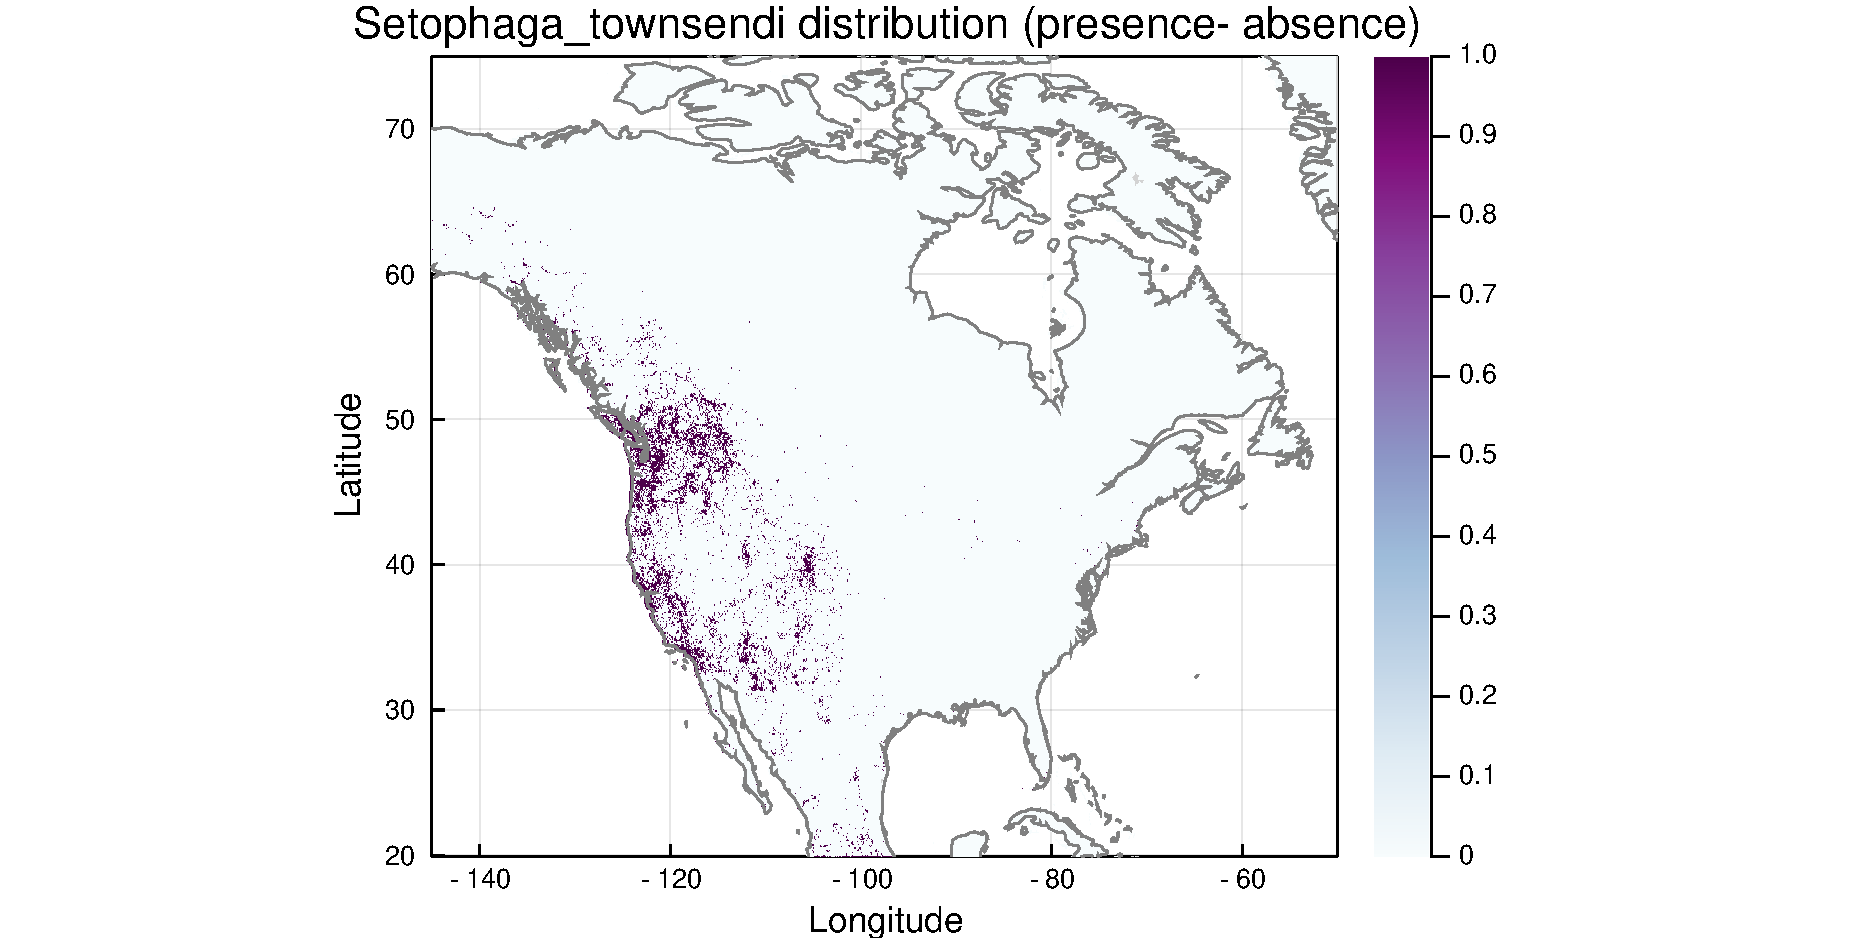
\includegraphics[scale=0.4]{fig/raw-sp-Setophaga_townsendi.pdf}
    \caption{Distribution des observations de la Paruline de Townsend (présence-absence)}
  \end{figure}
\end{frame}

\begin{frame}
  \frametitle{Données brutes - Matrice Y (non triée)}
  \begin{figure}
    \centering
    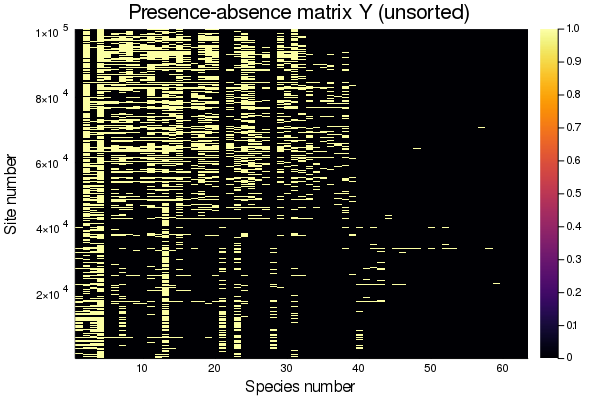
\includegraphics[scale=0.4]{fig/raw-Y-unsorted.png}
  \end{figure}
\end{frame}

\begin{frame}
  \frametitle{Données brutes - Matrice Y (triée par richesse, puis fréquence)}
  \begin{figure}
    \centering
    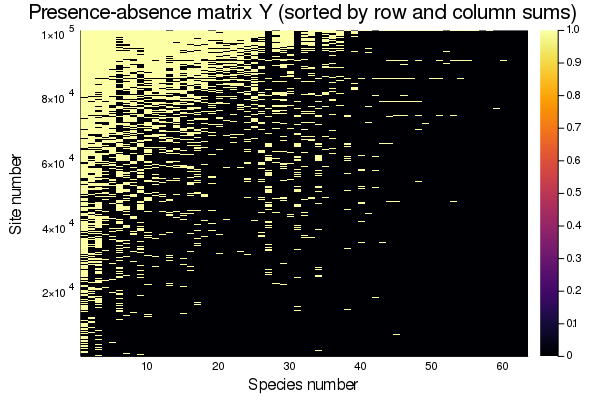
\includegraphics[scale=0.4]{fig/raw-Y-rowcolsorted.png}
  \end{figure}
\end{frame}

\begin{frame}
  \frametitle{Données brutes- Richesse spécifique (nombre d'espèces)}
  \begin{figure}
    \centering
    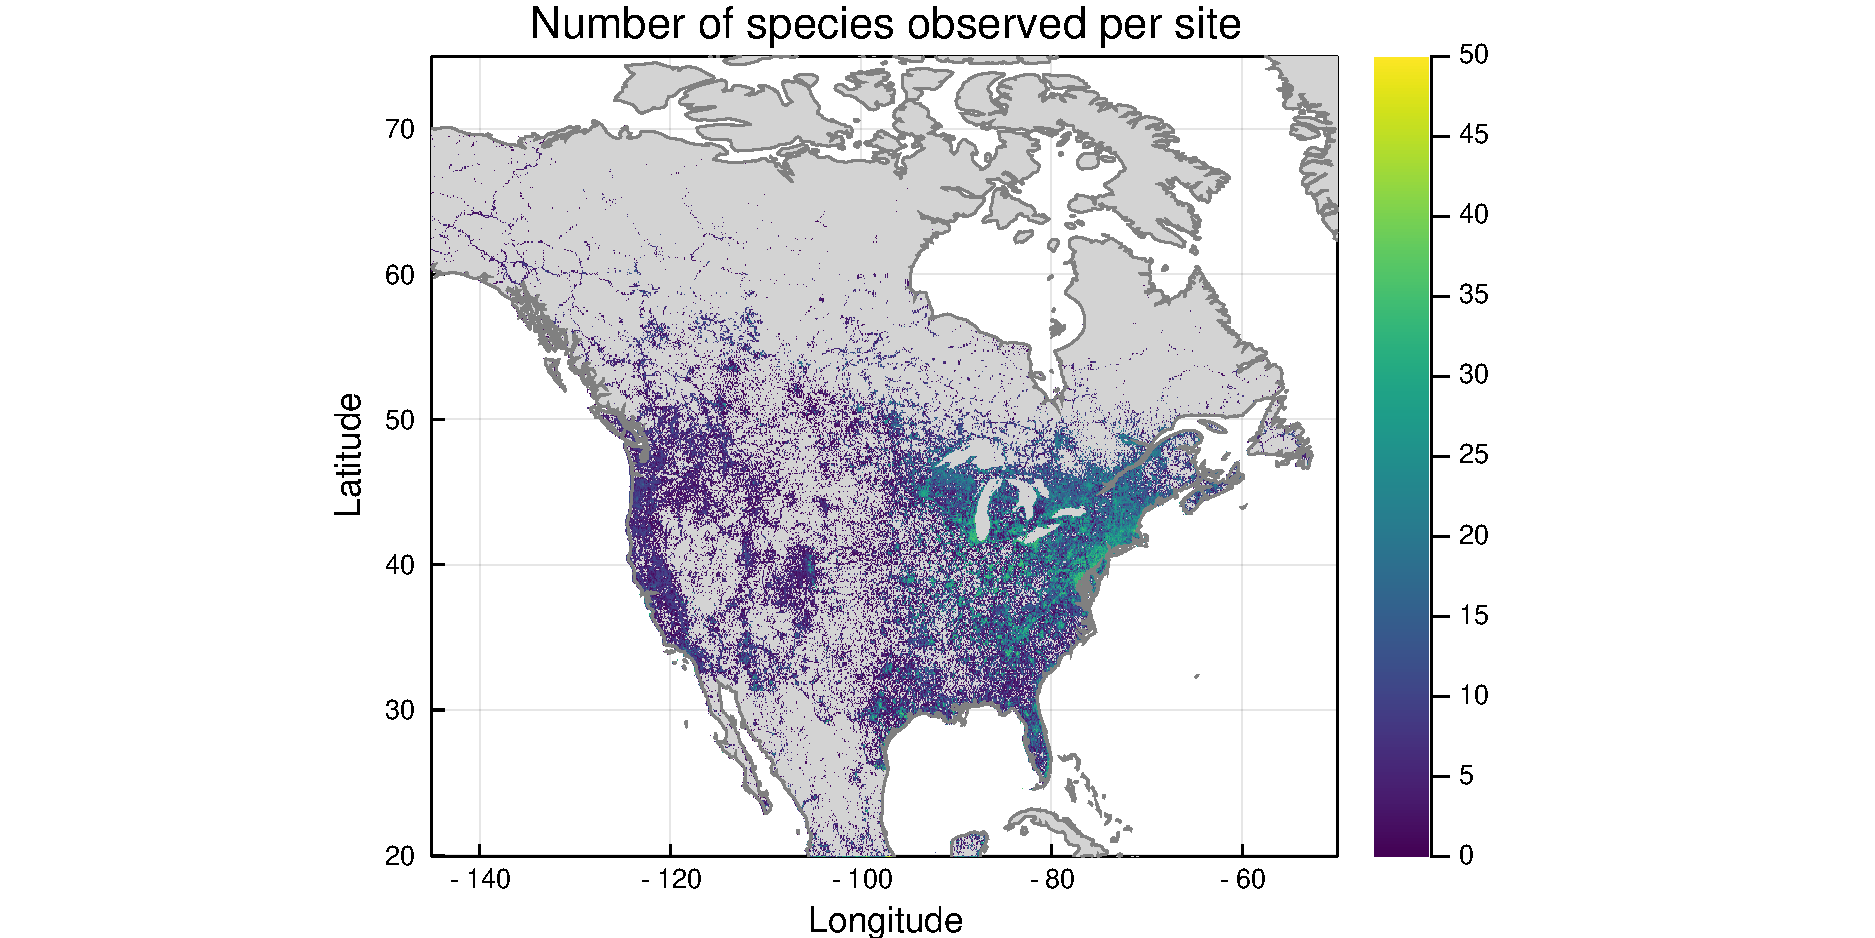
\includegraphics[scale=0.4]{fig/raw-richness.pdf}
  \end{figure}
\end{frame}

\begin{frame}
  \frametitle{Données brutes - Diversité spécifique}
  \begin{figure}
    \centering
    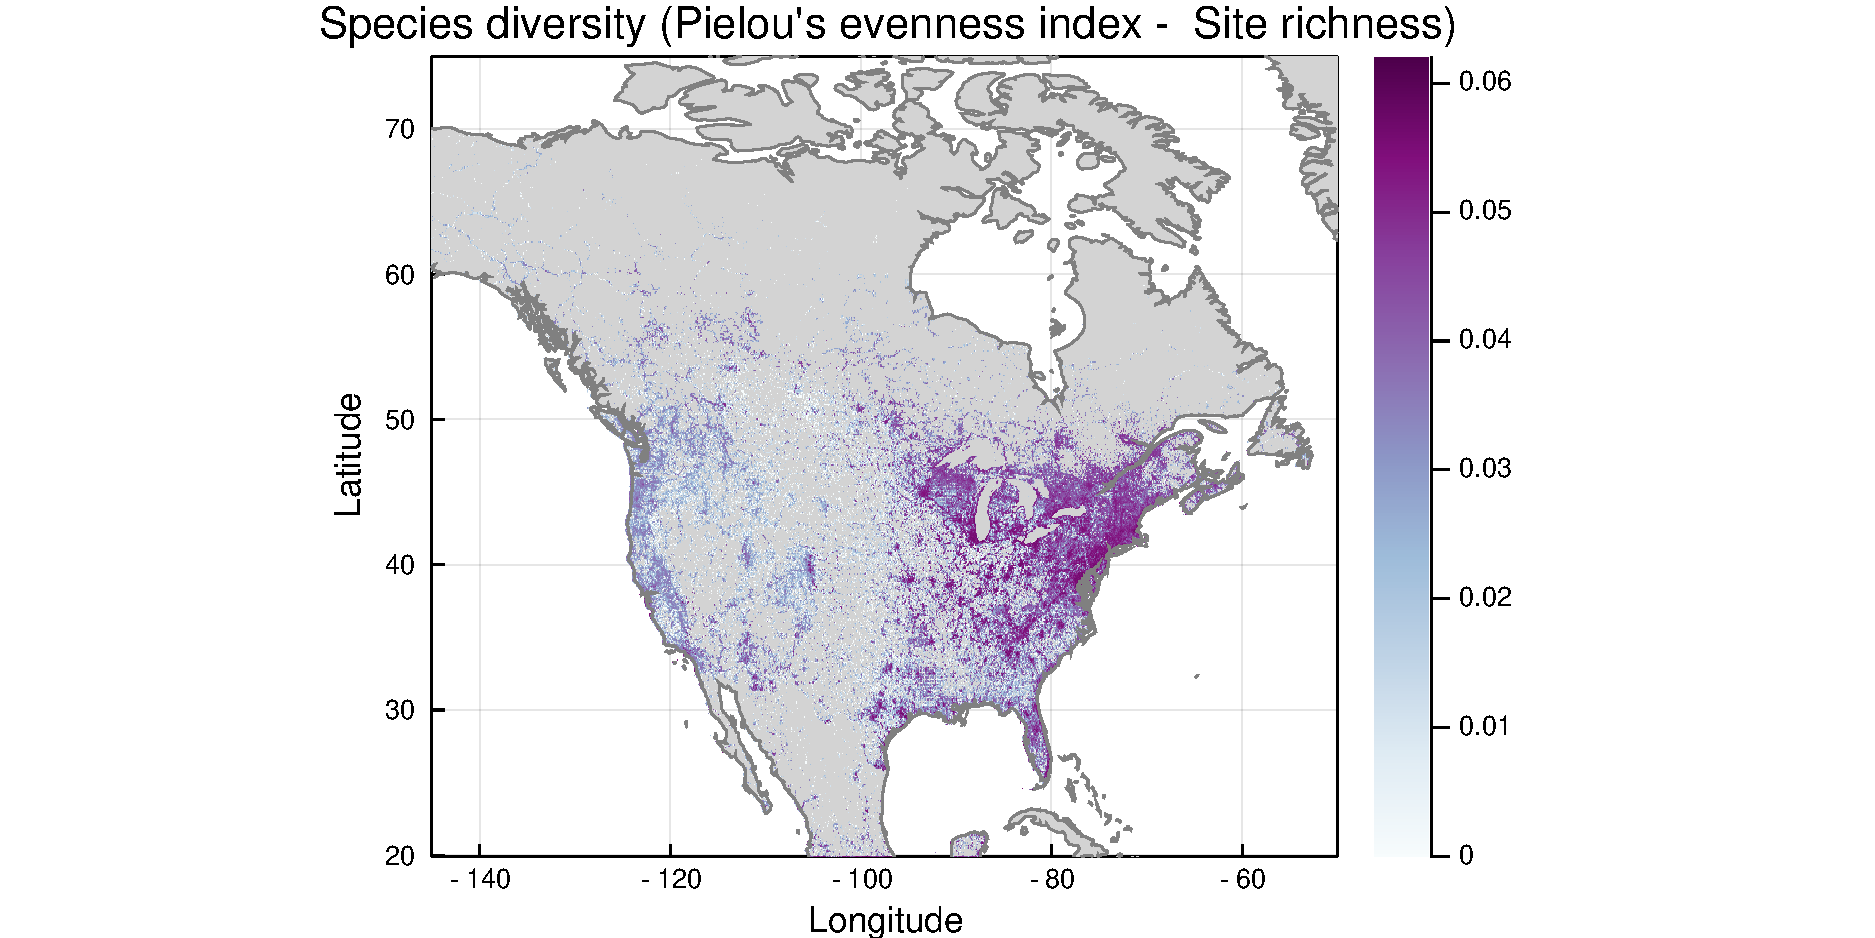
\includegraphics[scale=0.4]{fig/raw-diversity-pielou.pdf}
  \end{figure}
\end{frame}

\begin{frame}
  \frametitle{Données brutes - Diversité spécifique}
  \begin{figure}
    \centering
    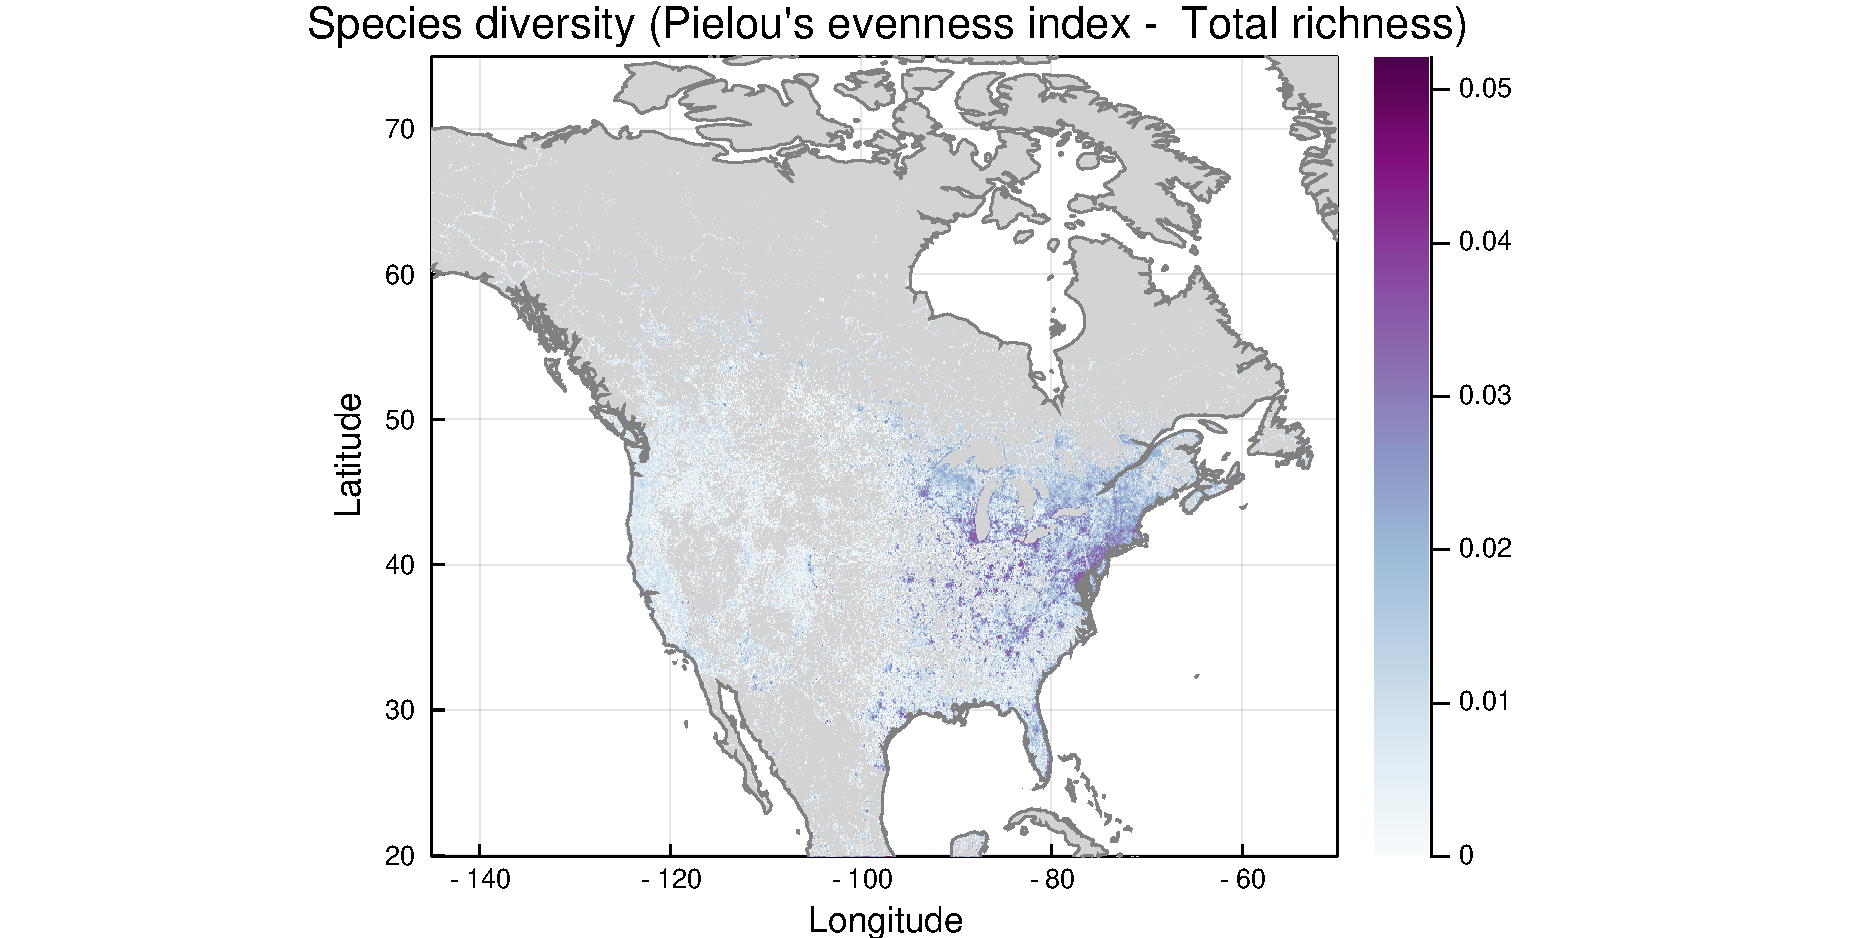
\includegraphics[scale=0.4]{fig/raw-diversity-pielou2.pdf}
  \end{figure}
\end{frame}

\begin{frame}
  \frametitle{Données brutes- LCBD}
  \begin{figure}
    \centering
    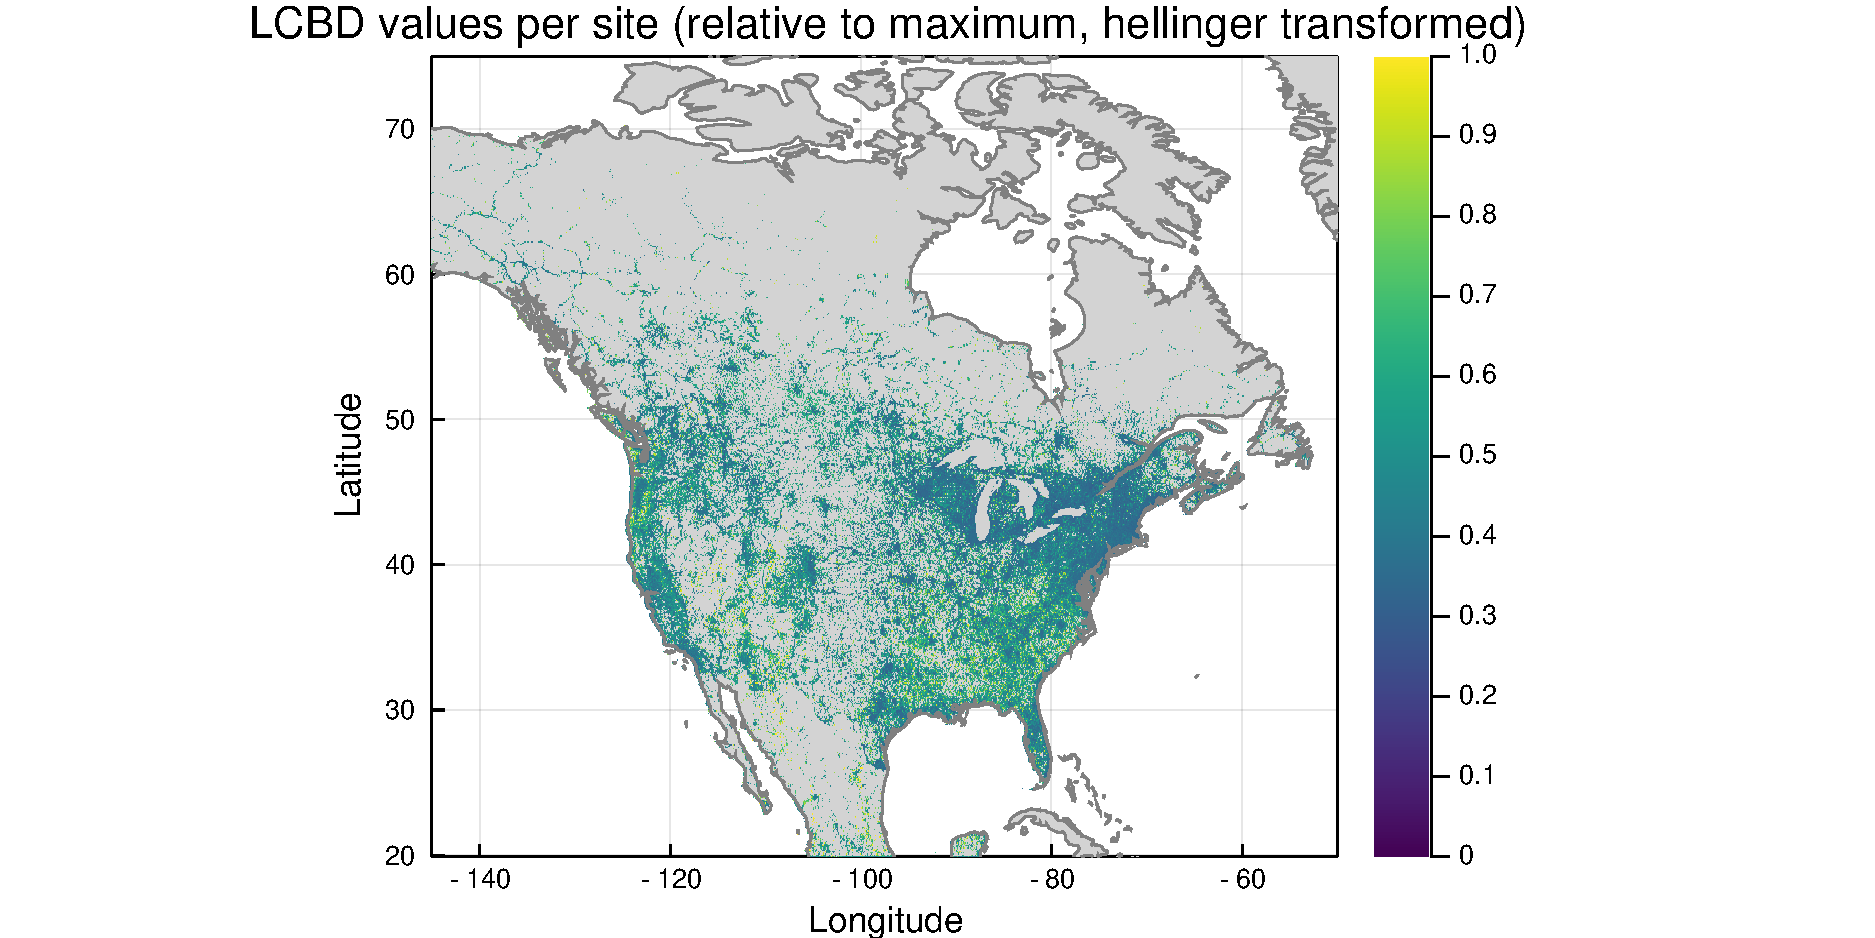
\includegraphics[scale=0.4]{fig/raw-lcbd-transf.pdf}
  \end{figure}
\end{frame}

\begin{frame}
  \frametitle{Données brutes - LCBD significatives}
  \begin{figure}
    \centering
    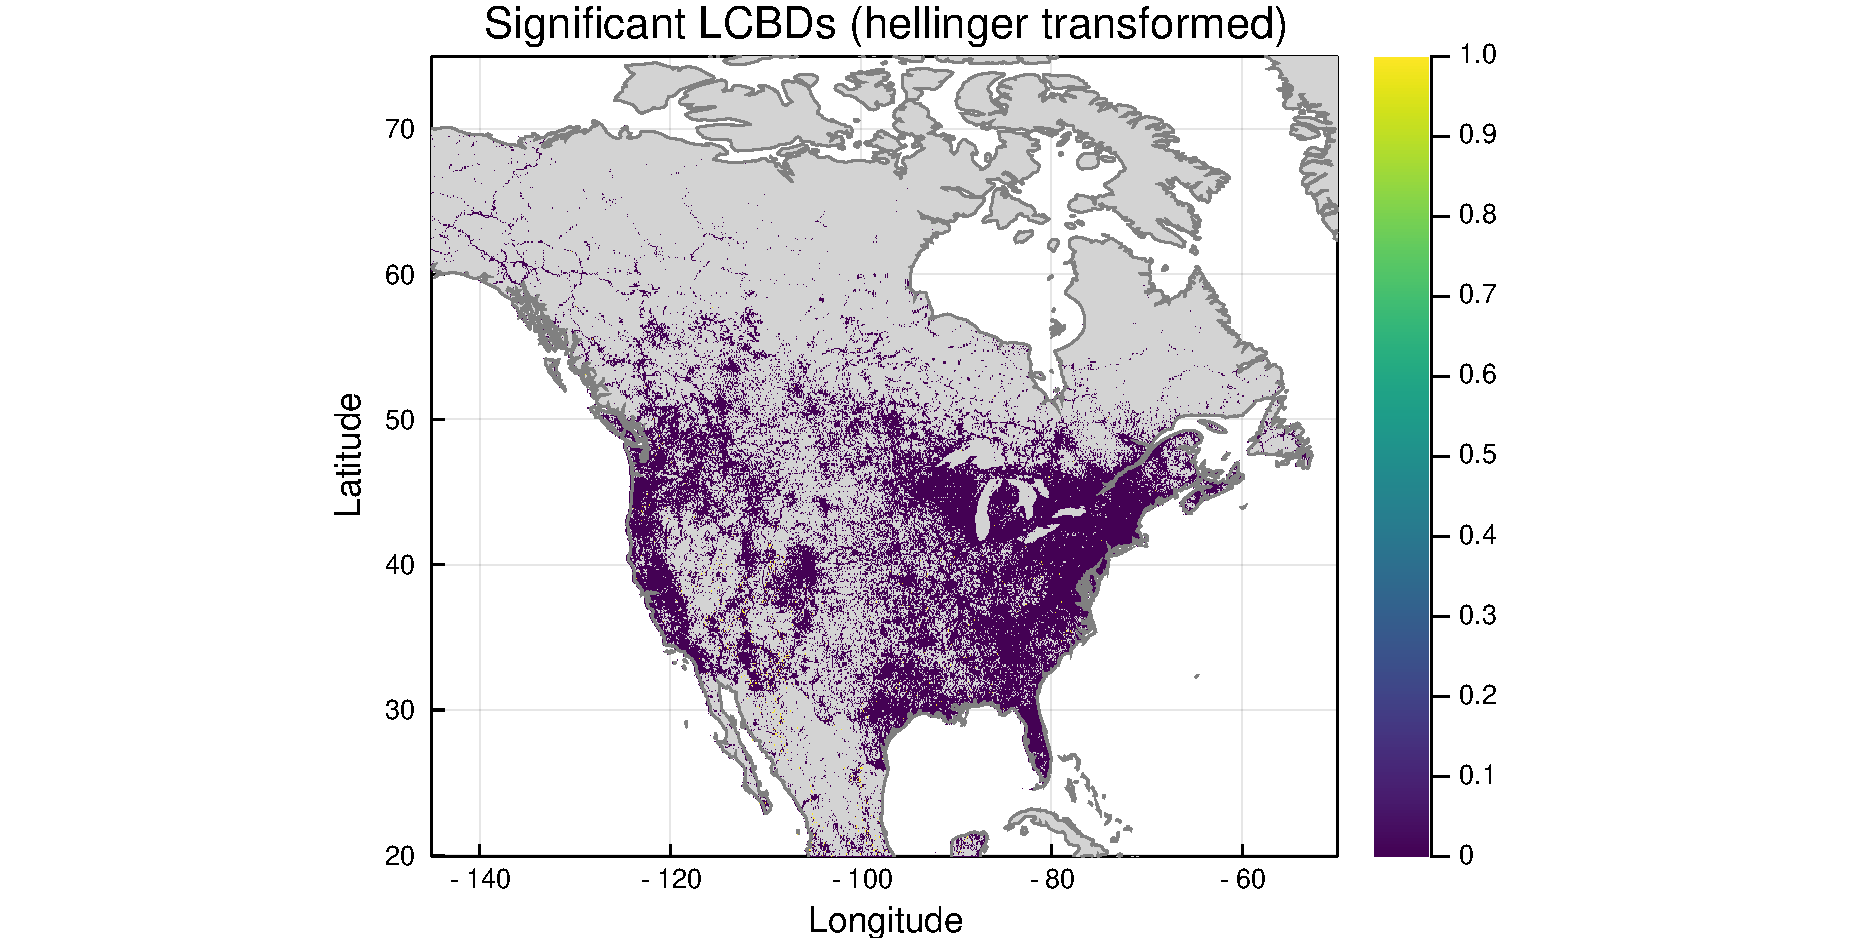
\includegraphics[scale=0.4]{fig/raw-lcbd-signif.pdf}
  \end{figure}
\end{frame}

\begin{frame}
  \frametitle{Données brutes - Relation LCBD-richesse}
  \begin{figure}
    \centering
    \includegraphics[scale=0.4]{fig/raw-lcbd-richness-transf.pdf}
  \end{figure}
\end{frame}

%%%%%%%%%%%%%%%%%%%%%%%%%%%%%%%%%%%%%%%%%%%%%%%%%%%%%%%%%%%%%%%%%%%%%

\begin{frame}
  \frametitle{SDM - 1 espèce, beaucoup d'observations}
  \begin{figure}
    \centering
    \includegraphics[scale=0.4]{fig/sdm-sp-Setophaga_petechia.pdf}
    \caption{Sortie du SDM pour la Paruline jaune}
  \end{figure}
\end{frame}

\begin{frame}
  \frametitle{SDM - 1 espèce, moins d'observations}
  \begin{figure}
    \centering
    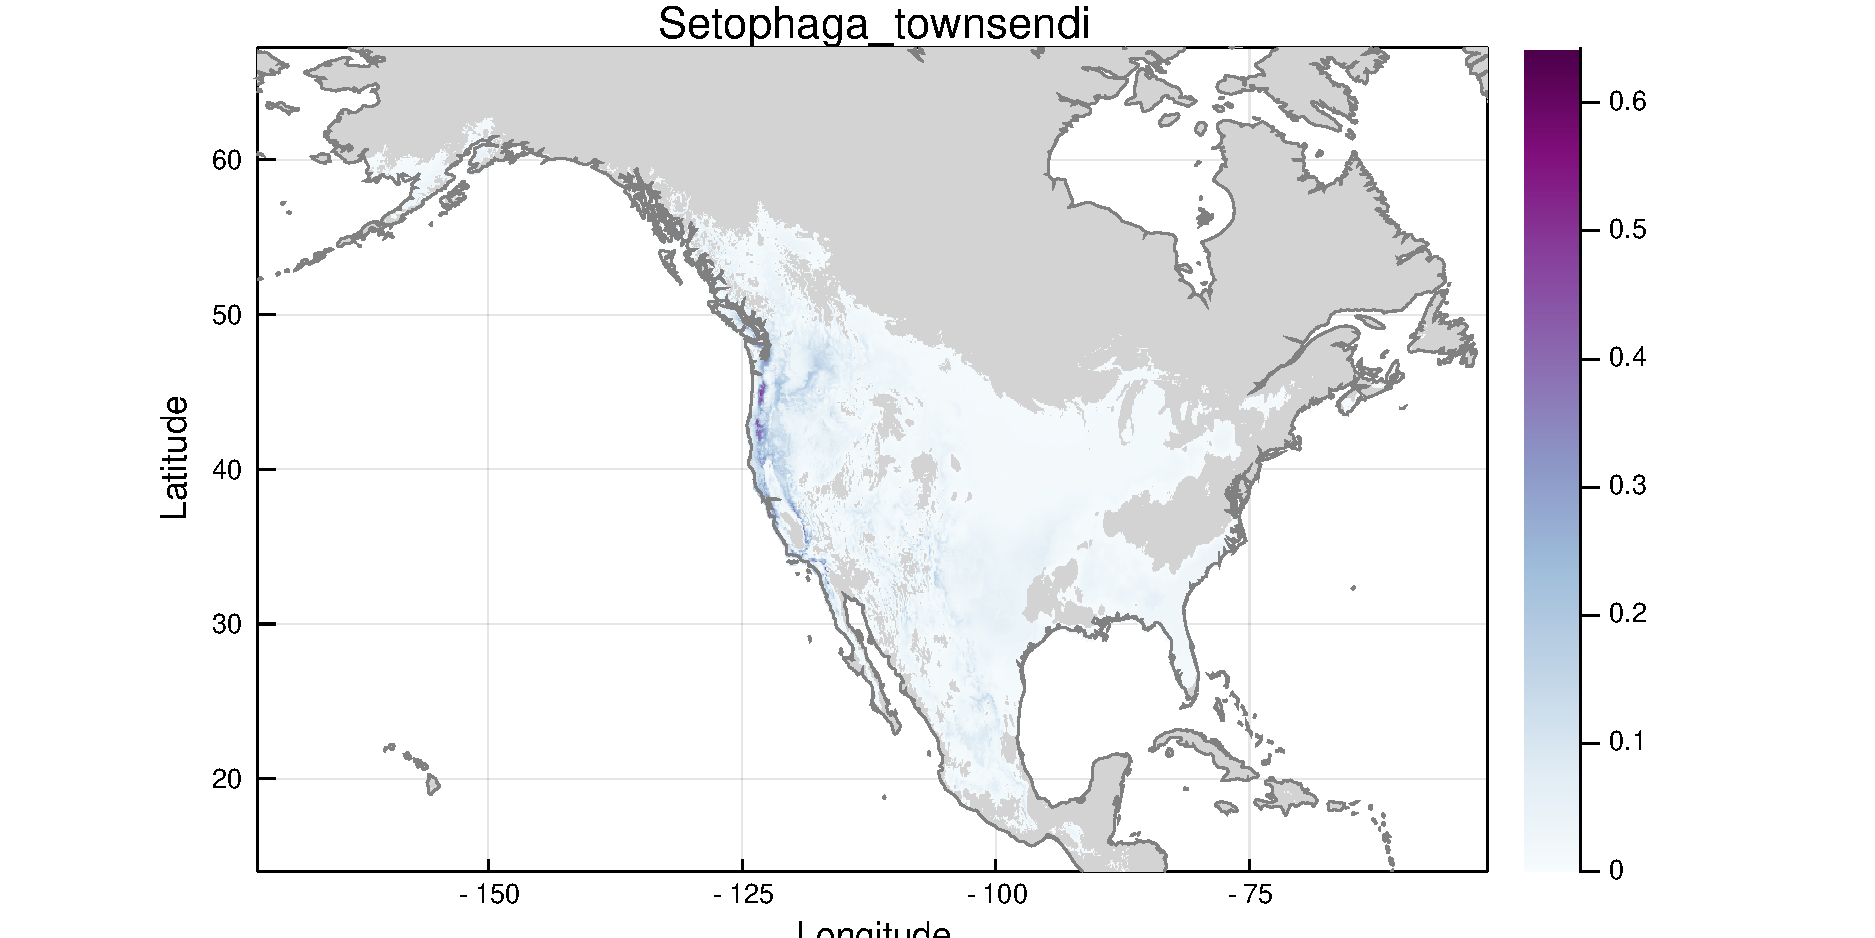
\includegraphics[scale=0.4]{fig/sdm-sp-Setophaga_townsendi.pdf}
    \caption{Sortie du SDM pour la Paruline de Townsend}
  \end{figure}
\end{frame}

\begin{frame}
  \frametitle{SDM - Matrice Y (non triée)}
  \begin{figure}
    \centering
    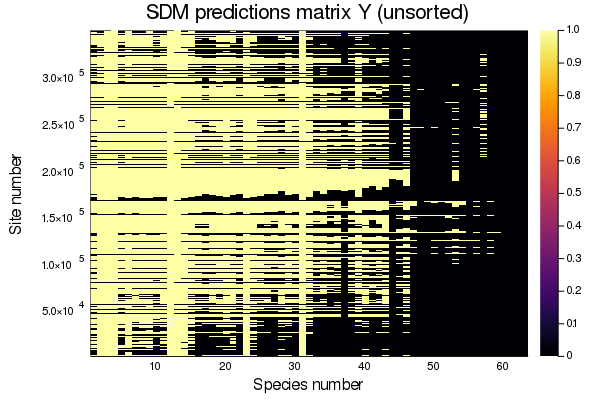
\includegraphics[scale=0.4]{fig/sdm-Y-unsorted.png}
  \end{figure}
\end{frame}

\begin{frame}
  \frametitle{SDM - Matrice Y (triée par richesse, puis fréquence)}
  \begin{figure}
    \centering
    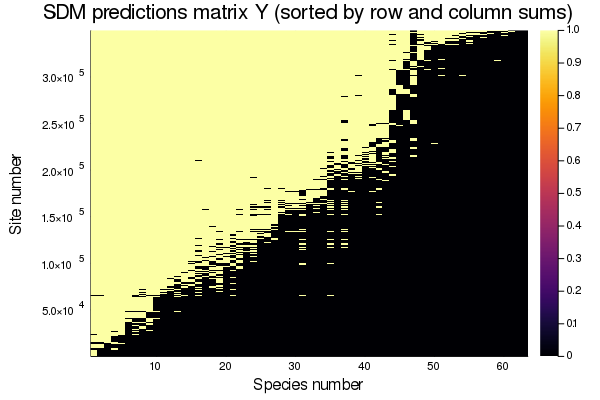
\includegraphics[scale=0.4]{fig/sdm-Y-rowcolsorted.png}
  \end{figure}
\end{frame}

\begin{frame}
  \frametitle{SDM- Richesse spécifique (nombre d'espèces)}
  \begin{figure}
    \centering
    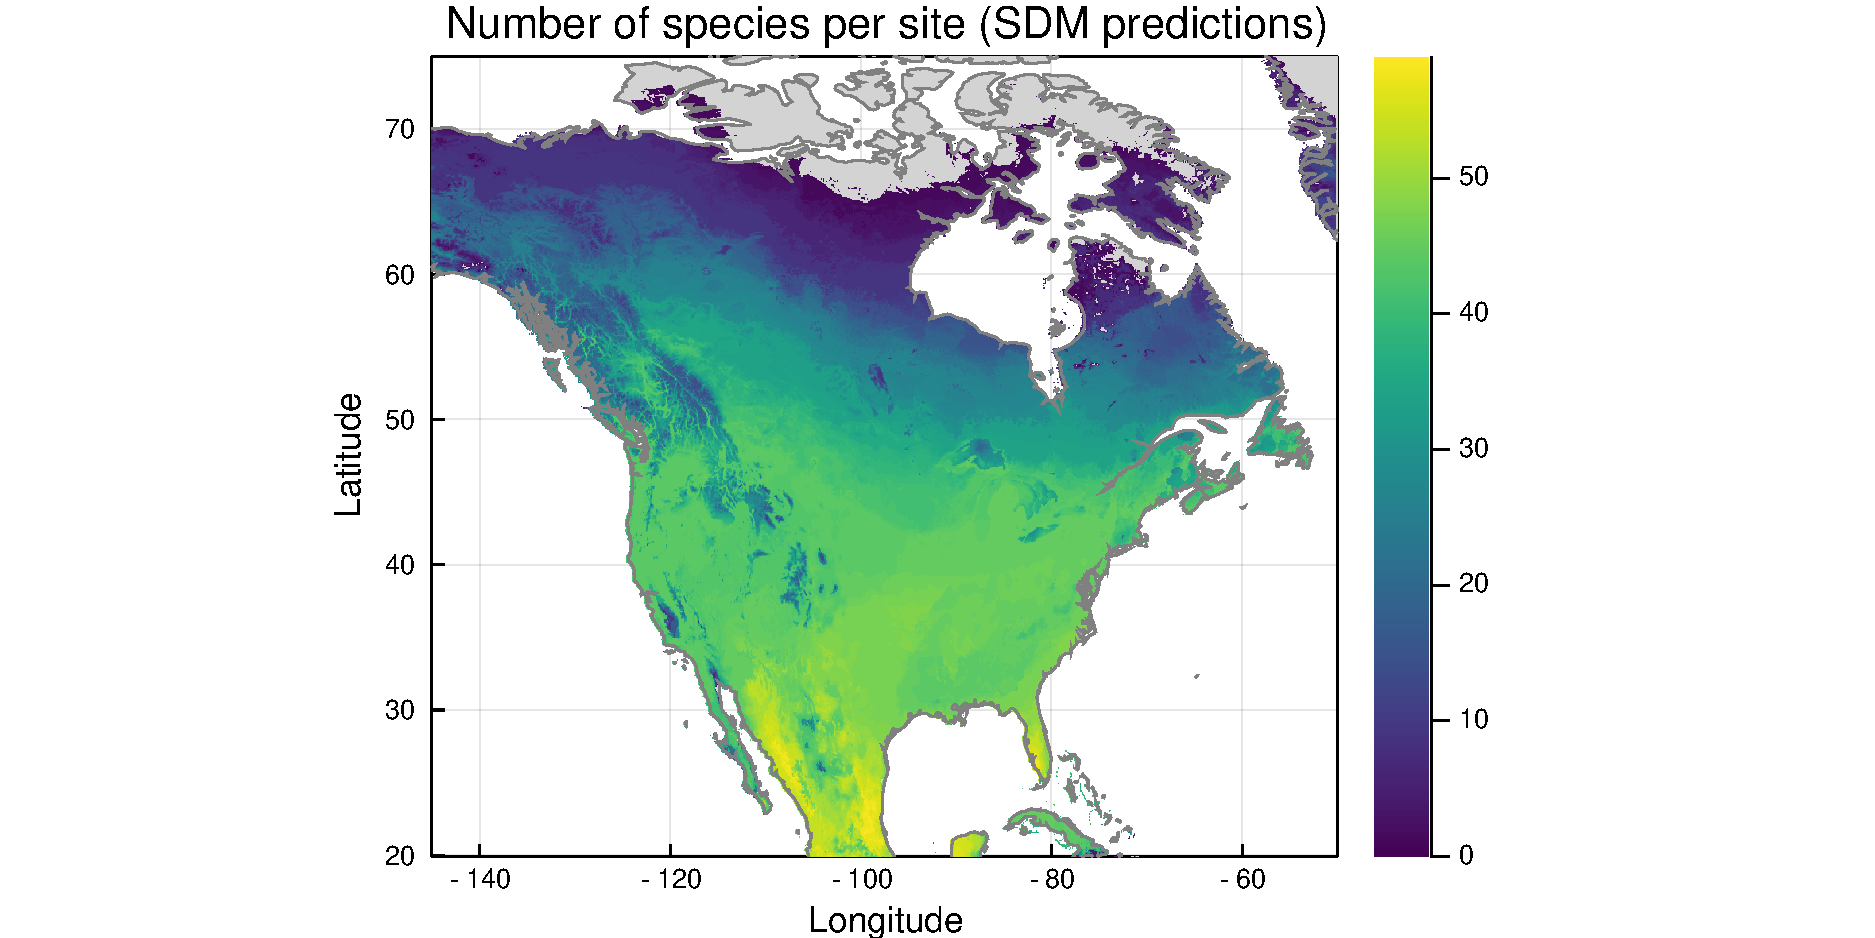
\includegraphics[scale=0.4]{fig/sdm-richness.pdf}
  \end{figure}
\end{frame}

\begin{frame}
  \frametitle{SDM - Diversité spécifique}
  \begin{figure}
    \centering
    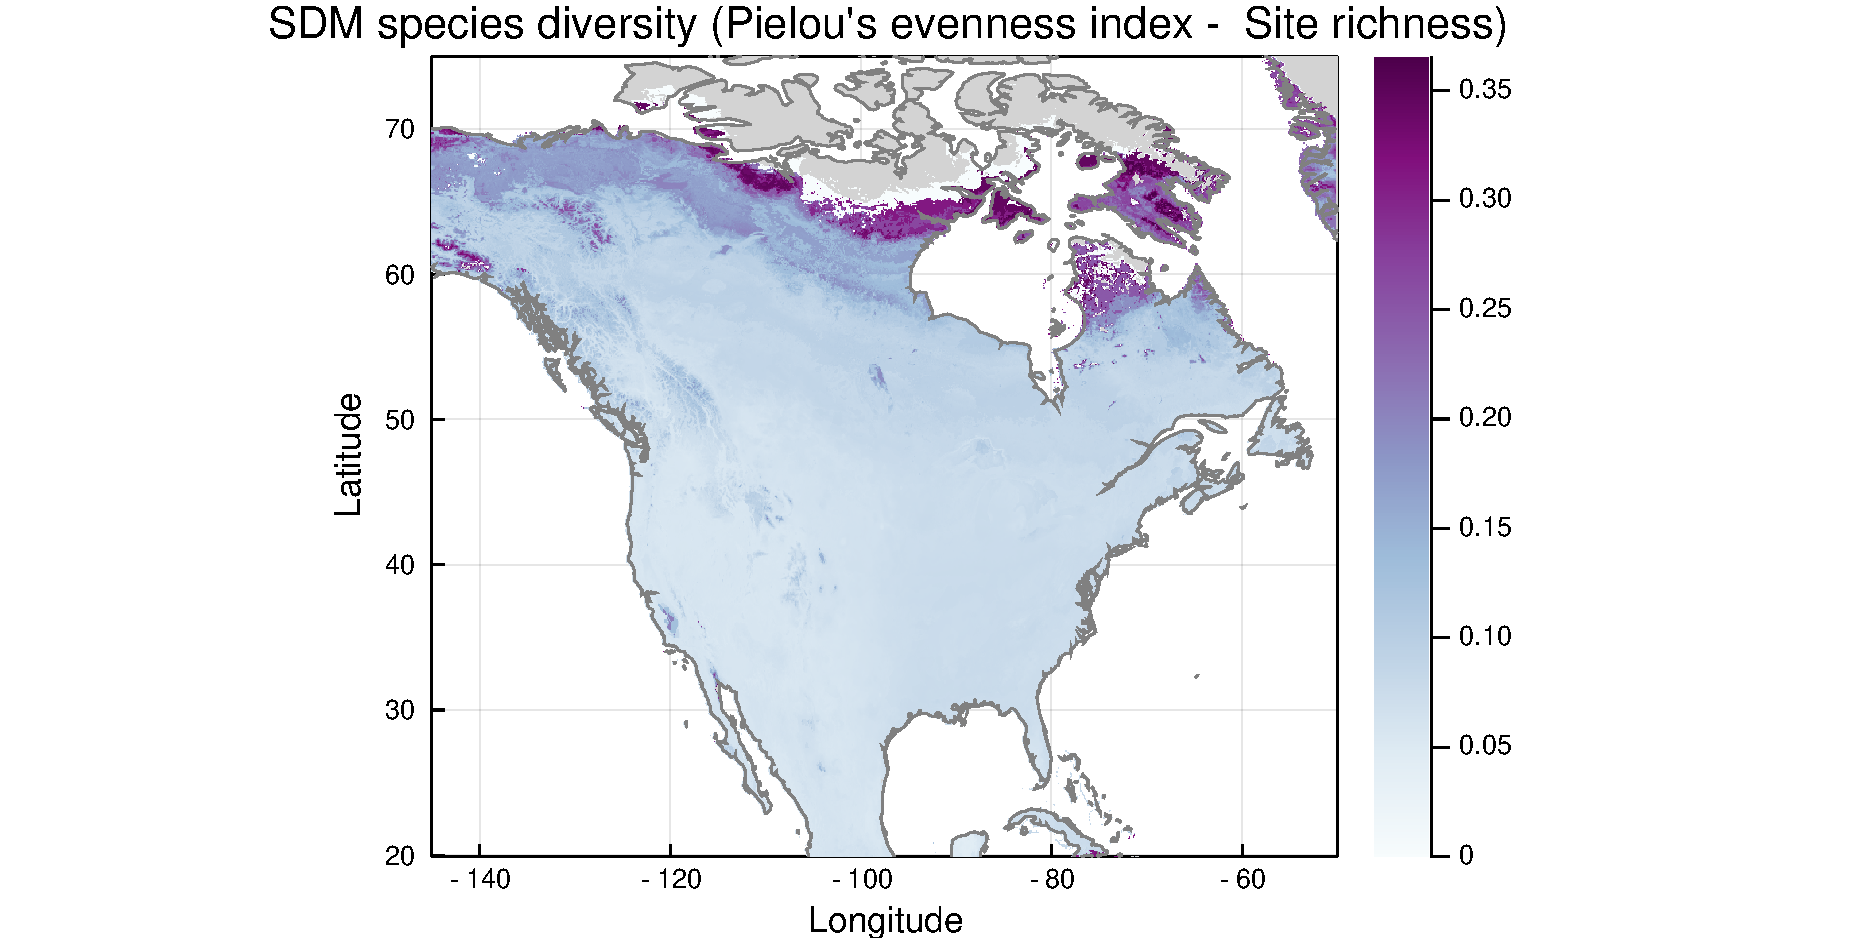
\includegraphics[scale=0.4]{fig/sdm-diversity-pielou.pdf}
  \end{figure}
\end{frame}

\begin{frame}
  \frametitle{SDM - Diversité spécifique}
  \begin{figure}
    \centering
    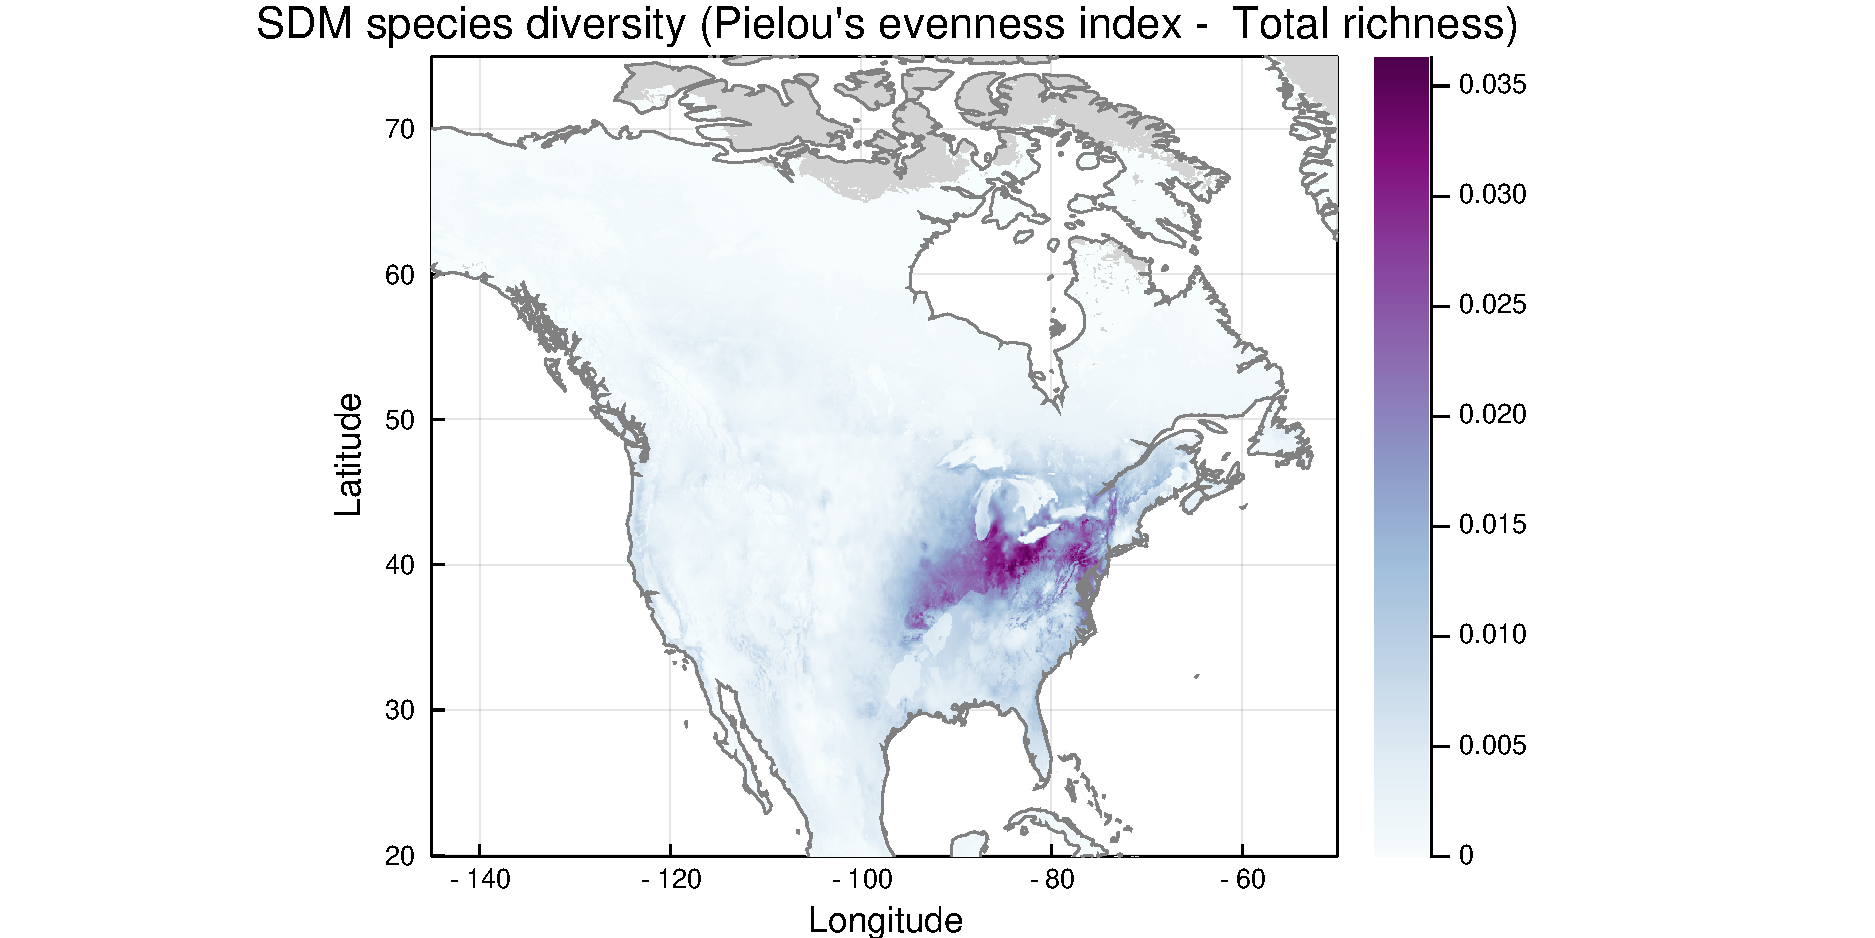
\includegraphics[scale=0.4]{fig/sdm-diversity-pielou2.pdf}
  \end{figure}
\end{frame}

\begin{frame}
  \frametitle{SDM - LCBD}
  \begin{figure}
    \centering
    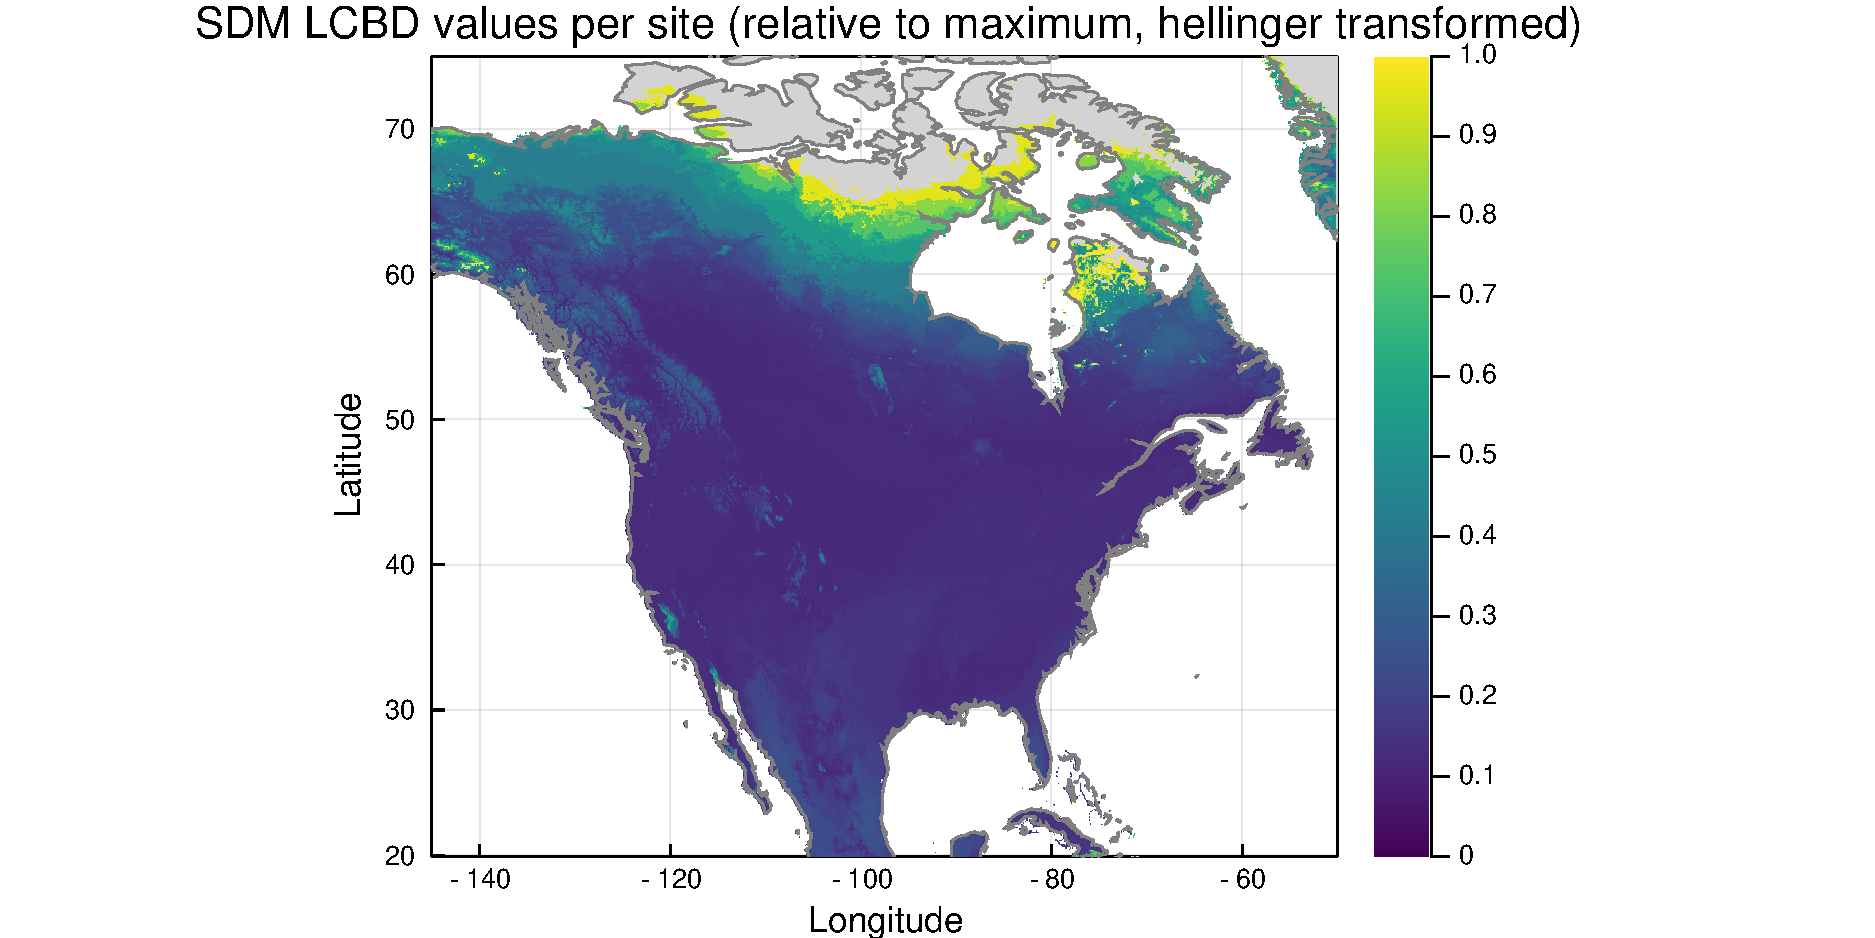
\includegraphics[scale=0.4]{fig/sdm-lcbd-transf.pdf}
  \end{figure}
\end{frame}

\begin{frame}
  \frametitle{SDM - LCBD significatives}
  \begin{figure}
    \centering
    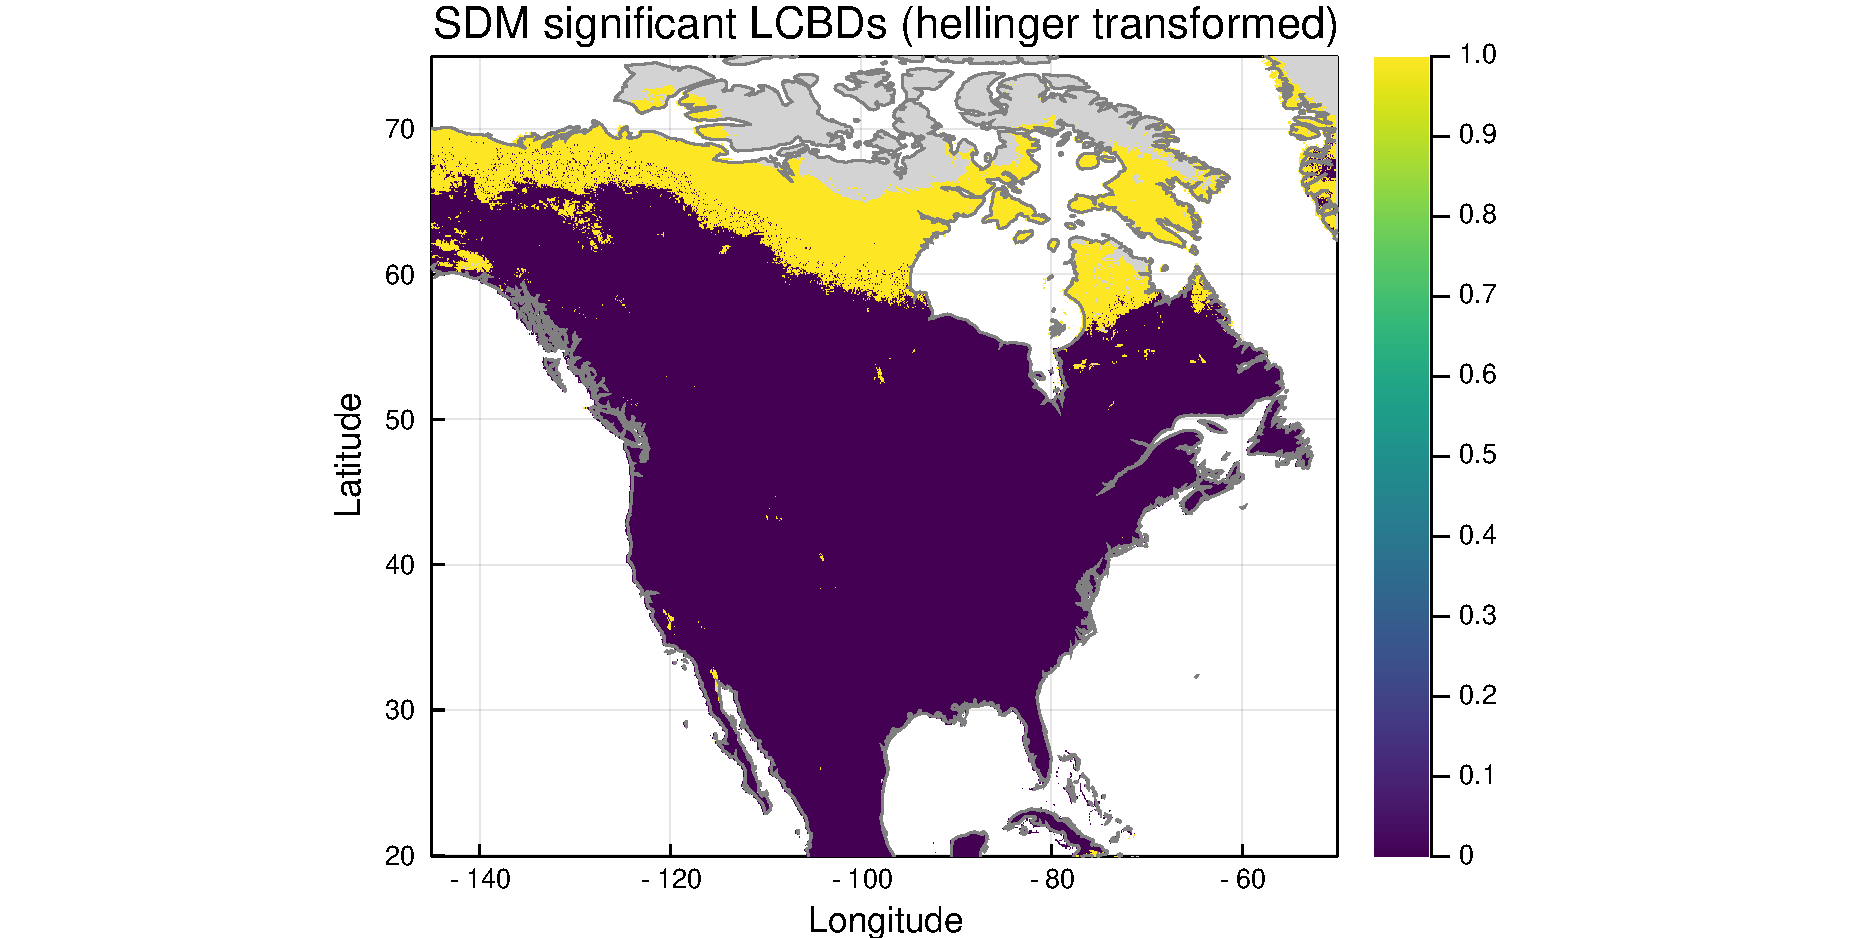
\includegraphics[scale=0.4]{fig/sdm-lcbd-signif.pdf}
  \end{figure}
\end{frame}

\begin{frame}
  \frametitle{SDM - Relation LCBD-richesse}
  \begin{figure}
    \centering
    \includegraphics[scale=0.4]{fig/sdm-lcbd-richness-transf.pdf}
  \end{figure}
\end{frame}

\end{document}
